\documentclass[conference]{IEEEtran}
\usepackage[utf8]{inputenc}
\usepackage{amsmath}
\usepackage{amsfonts}
\usepackage{amssymb}
\usepackage{graphicx}
\usepackage{hyperref}
\usepackage{bookmark}
\usepackage{xcolor}
\usepackage{algpseudocode}
\usepackage{algorithm}
\usepackage{cite}

\title{Reinforcement Learning for Rocket League (RL$^2$)}
\author{
    \IEEEauthorblockN{Anshuman Dash, Phillip Peng, Matthew Shen}
    \IEEEauthorblockA{
        Department of Computer Science\\
        University of California, Santa Barbara\\
        Email: \{anshumandash, plp, matthewshen\}@ucsb.edu
    }
}
\date{Winter 2025}


\begin{document}

\maketitle

\begin{abstract}
We aim to investigate the use of Reinforcement Learning in the context of the game of Rocket League. Through the uses of PPO and Curriculum Learning through self-play, we train bots on a variety of reward structures and hyperparameters. To do an empirical comparison of the different models, we evaluate the bots against each other in a tournament setting of 1v1 matches to determine model ELO. We analyze the results of this tournament as well as individual models and discuss the implications of our findings.
\end{abstract}

\section{Introduction}
Reinforcement Learning (RL) is a powerful tool for training agents to perform tasks in a variety of environments. We aim to investigate the use of RL in the context of the game of Rocket League. Rocket League is a popular video game that combines soccer with rocket-powered cars. The game is played in a 3D environment, and players control their cars to hit a ball into the opposing team's goal. The game itself holds a large number of states making it a challenging environment for RL agents to learn in. 

\section{Related Work}
The use of RL to play games has been a popular research topic in recent years, most famously with AlphaGo. The application of RL in other games such as Dota 2 and Starcraft II has also been explored. 


\subsection{Proximal Policy Optimization (PPO)}
Throughout all of our trianing, we use Proximity Policy Optimizaiton (PPO) as our training algorithm. a;lsjdfl;asdfflsf Explain structure a;lksdfj;lasdjf;lasf. The pseudo code for PPO can be seen in Algorithm \ref{alg:PPO}.

\[
    L_{\theta_k}^{\text{CLIP}} = \hat{\mathbb{E}}_t\left\{ \text{min}(r_t(\theta)\hat{A}_t, \text{clip}(r_t(\theta), 1-\epsilon, 1+\epsilon)\hat{A}_t)\right\}
\]

\begin{algorithm}
    \begin{algorithmic}[1]
        \State \textbf{Input:} initial policy parameters $\theta_0$, initial value function parameters $\phi_0$
        \For {k = 0,1,2, ... } 
        \State Collect set of trajectories $\mathcal{D}_k$ by running policy $\pi_k = \pi(\theta_k)$ in the environment
        \State Compute rewards-to-go $\hat{R}_t$ 
        \State Compute advantage estimates $\hat{A}_t$ for current value function $V_{\phi_k}$
        \State Update policy by maximizing PPO-Clip objective:
        \State \hspace{1cm} $\theta_{k+1} = \arg\underset{\theta}{\max} \mathcal{L}_{\theta_k}^{\text{CLIP}}$
        \State Fit value function by regression on mean-squared error:
        \State \hspace{1cm} $\phi_{k+1} = \arg\underset{\phi}{\min}{\phi} \hat{\mathbb{E}}_t\left\{ (V_{\phi}(s_t) - \hat{R}_t)^2 \right\}$
        \EndFor
    \end{algorithmic}
    \caption{Pseudocode for the Proximal Policy Optimization (PPO) algorithm. The algorithm iteratively updates the policy and value function parameters to maximize the expected reward while ensuring the updates do not deviate too much from the previous policy in the positive direction.}
    \label{alg:PPO}
\end{algorithm}

\section{Implementation Details}
 The agent's observation space consists of the current state of the game, which includes but is not limited to the positions and velocities of the cars and ball, as well as boost pad locations. This reduces down to a 89 dimensional tensor. The action space consists of 8 multi-discrete actions which include the ability to move cardinally, jump, boost, drift and dodge. 

 We implement and train the agents through a package called RLGym which allows the training of Rocket League agents.




\section{Model and Methods}
Through this work we largely explore how a change in reward structure as well as model hyperparameters affect the performance of trained agents. All models are trained using the Proximal Policy Optimization (PPO) algorithm.

\subsection{Reward Scaling}


\subsection{Reward Structures}

\subsection{Curriculum Learning}
Curriculum learning is a training strategy where the learning process is organized in a way that gradually increases in complexity. We first attempted to implement this in the context of Rocket League by starting with a simple reward structure and gradually increasing the complexity of the reward structure as the agents learn.

We find that this doesn't perform well for a variety of reasons. The increasing sparsification of rewards makes it difficult for the agents to learn effectively. In order to address this, we propose a modified approach that balances exploration and exploitation.

We then attempted to implement an automatically updating curriculum learning strategy, which would automatically scale rewards based on the number of training steps that have occurred. 

\[
    if 
        r_t = \frac{1}{n}
\]

\subsection{Common Pitfalls}
In the beginning of the project, we encountered a number of pitfalls that made training difficult. One such pitfall was the use of a constant negative reward for the agent. This is intutive as it would encourage the agent to score goals sooner to prevent the occurance of the negative reward. However, in practice, we found that this more often than not led the agent to simply allow the opponent to score a goal to stop incurring the negative reward. This can be seen as a form of reward hacking, where the agent finds a way to exploit the reward structure to maximize its reward. This could theoretically be fixed by scaling this constant reward down, however we decided to remove it entirely from our reward structure.

\begin{figure}
    \centering
    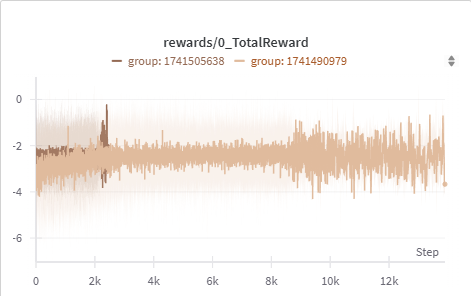
\includegraphics[width=\linewidth]{images/Phase0-TotalReward.png}
    \caption{\textbf{Total reward over time for a model trained with a constant negative reward:} Constant Negative Reward at every timestep resulted in an overall negative reward. This resulted in a form of reward hacking where the agent would allow the opponent to score to stop incurring negative reward.}
    \label{fig:phase0-totalreward}
\end{figure}

The thought of using a pure goal oriented reward structure may also seem intutive. This can be especially seen in the reward structure of \textcolor{blue}{AlphaGo}. However, in the context of Rocket League, this is not effective as the state-action space is so large and without a method such as Monte Carlo Tree Search (MCTS) as in AlphaGo, it makes each state exceptionally sparse in terms of reward, making it difficult for the agent to learn effectively. We train a model with a pure goal oriented reward structure for 700 million timesteps to show the ineffectiveness of this reward structure. 



\section{Results}
We evaluate the performance of the trained agents by having them play against each other in a Placket Luce tournament



\section{Future Work}
Due to time constraints of the project most of the models were trained in the order of tens to hundreds of million timesteps, while most high level play bots, are trained in the order of billions of timesteps. Additionally, the majority of bots are not incentivised to use some inherent features of the space, such as boost and the space in the air. Exploring whether these features still apply to models trained for longer periods of time uses these features would be an interesting analysis. 

Additionally we initially aimed to explore the use of methods such as \textcolor{blue}{Hierarchical Reinforcement Learning, Model distillation, and Network Distillation} and their effect on model performance. Hierarchical Learning requires a good low-level policy to be able to be effective before training higher level policies which would require having a good low-level policy early on. Model distillation suffers from the same drawback of needing some initial good policy to distill from. \textcolor{red}{On the case of Network Distillation, we just ran out of time lmao.}

Lastly implementing a more accurate form of self-play woudl be beneficial. Currently models are trained only against its current self, which can lead to a lack of diversity in training data. Implementing self-play where the model plays against a variety of past versions of itself would improve this significantly.

\section{Conclusion}


\cite{sigal2023improving}

dfadsf \cite{zhang2019hierarchical}

 adsfasd \cite{shao2019survey}

%  asdf \cite{Oh2022Fighting}

asdf \cite{vinyals2017starcraft}

\cite{Pleines2022RocketSimDRL}

\cite{Misaros2024RocketPPO}

\cite{Albuainain2020RLPhysics}


\bibliographystyle{IEEEtran}
\bibliography{references}

\end{document}

